% Final report, LMA Group Project (CL3.410, Monsoon 2026), Team Disco 82.
% Build:  cd docs/report && pdflatex final_report.tex && pdflatex final_report.tex
% Every number below comes from files on main: docs/results.md, results/summary/*, data/mining_report.md,
% docs/extension_results.md and PREREGISTRATION.md.
\documentclass[10pt,a4paper]{article}
\usepackage[a4paper,margin=2cm]{geometry}
\usepackage[T1]{fontenc}
\usepackage{lmodern}
\usepackage{mathptmx}
\usepackage[scaled=0.88]{helvet}
\usepackage{microtype}
\usepackage{booktabs}
\usepackage{tabularx}
\usepackage{array}
\usepackage[table]{xcolor}
\usepackage{enumitem}
\usepackage{caption}
\usepackage{titlesec}
\usepackage{multicol}
\usepackage{float}
\usepackage[hidelinks]{hyperref}
\usepackage{tikz}
\usetikzlibrary{positioning,arrows.meta}

\setlist{nosep,leftmargin=*}
\setlength{\parskip}{3pt}
\setlength{\parindent}{0pt}
\captionsetup{font=small,labelfont=bf,skip=3pt}
\titlespacing*{\section}{0pt}{8pt}{3pt}
\titlespacing*{\subsection}{0pt}{6pt}{2pt}
\titleformat*{\section}{\large\bfseries}
\titleformat*{\subsection}{\normalsize\bfseries}
\newcolumntype{Y}{>{\raggedright\arraybackslash}X}
\newcommand{\code}[1]{\texttt{\small #1}}
\newcommand{\m}{$-$}
\renewcommand{\arraystretch}{1.08}

\begin{document}

\begin{center}
{\LARGE\bfseries Run It, Then Cite It: Execution- and Mutation-Verified\\[2pt] Answers to Developer Questions}\\[6pt]
{\large Ameya Purohit, Sunil Kumar, Aditya Narayan Dwivedi, Sourav Nath}\\[2pt]
LMA Group Project (CL3.410, Monsoon 2026), Team Disco 82\\[2pt]
\small Code, data and reproduction steps: \url{https://github.com/ameya-purohit/LMA-Final-Project}
\end{center}

\begin{abstract}
\noindent Developers often ask how a library really behaves when its documentation may be wrong. LLM assistants tend
to repeat the documentation and cite code that looks related but does not decide the behaviour. We built an agent that
checks its own answer twice: it runs a small test program for each claim, and it keeps a cited code line only if
changing that line changes the test's result. We compared it with a ReAct agent that had the same tools, model and
budget, on 145 real GitHub issues from \code{click} and \code{marshmallow}, with answer keys built automatically from
each issue's merged fix. The hypotheses were pre-registered and the test set was locked before any test run. Our agent
did \textbf{not} win: 40.0\% of its answers were correct and correctly cited, against 49.7\% for ReAct by an LLM
judge, and 25.0\% against 41.7\% on 12 questions labelled by humans. The line-changing check was the main problem: it
rejected most of the lines that developers actually fixed. Both agents were far better than simple baselines, and no
system ran an unsafe action.
\end{abstract}

\section{Introduction}

``Why does this library behave differently from its documentation?'' is a common developer question. The answer
usually depends on code spread across files: where a default is set, where it is overridden and which branch runs.
LLMs answer such questions confidently and often repeat the documentation even when the code disagrees. Agents that
search and read code do better, but they still decide behaviour by \emph{reading}, and LLMs misread control flow and
overrides. A second, less visible problem is citations. An answer can cite lines that are on topic but do not
produce the behaviour. Code gives us a test that plain text does not have: run the behaviour, change the cited line,
and see whether the behaviour changes.

Our agent (``ours'') adds two checks to a tool-using code agent. \textbf{Check 1, run it:} every behavioural claim in
a draft answer is tested by a probe in a sandbox, and a refuted claim is investigated again with the observed output
as the new goal. \textbf{Check 2, flip the switch:} every citation of a confirmed claim is mutated (a constant
changed, a condition negated, a comparison swapped, a statement deleted). The citation is accepted as \emph{causal}
only if some mutant changes the claim probe's result and leaves the control probes unchanged. A rejected citation
sends the agent looking for the line that does decide the behaviour. Each final claim carries a grade: executed and
causally cited (E+C), executed (E), confirmed by a repository test (T), read only (R) or documentation only (D).
Figure~\ref{fig:loop} shows the loop.

\begin{figure}[H]
\centering
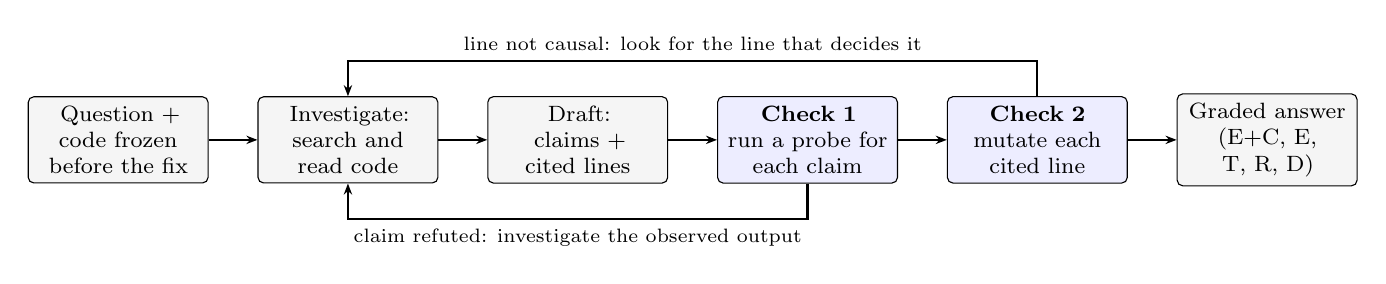
\begin{tikzpicture}[font=\footnotesize, node distance=0.62cm,
  box/.style={draw, rounded corners=2pt, align=center, text width=2.05cm, minimum height=1.05cm, fill=gray!8},
  chk/.style={box, fill=blue!7},
  arr/.style={-{Stealth[length=4pt]}, thick}]
\node[box] (q) {Question +\\code frozen before the fix};
\node[box, right=of q] (inv) {Investigate:\\search and read code};
\node[box, right=of inv] (dr) {Draft:\\claims + cited lines};
\node[chk, right=of dr] (c1) {\textbf{Check 1}\\run a probe for\\each claim};
\node[chk, right=of c1] (c2) {\textbf{Check 2}\\mutate each\\cited line};
\node[box, right=of c2] (ans) {Graded answer\\(E+C, E, T, R, D)};
\draw[arr] (q)--(inv); \draw[arr] (inv)--(dr); \draw[arr] (dr)--(c1);
\draw[arr] (c1)--(c2); \draw[arr] (c2)--(ans);
\draw[arr] (c1.south) -- ++(0,-0.45) -| node[pos=0.25,below,font=\scriptsize]{claim refuted: investigate the observed output} (inv.south);
\draw[arr] (c2.north) -- ++(0,0.45) -| node[pos=0.25,above,font=\scriptsize]{line not causal: look for the line that decides it} (inv.north);
\end{tikzpicture}
\caption{The agent's loop. Confirmed claims go on to Check 2, and causal lines go into the answer. Failed checks send it back to investigate; budget limits stop the loop (8 investigation
steps, 12 probe runs, 25 requests per question).}
\label{fig:loop}
\end{figure}

\textbf{Research questions.} RQ1: does this procedure give more correct, causally cited answers, and fewer confident
errors, than a ReAct agent with the same tools (including execution and mutation) and the same limits? RQ2: how well
does the mutation check agree with human judgements of causality and with the lines the developer changed, and which
acceptance rule agrees best?

\begin{center}
\fbox{\begin{minipage}{0.97\linewidth}\small
\textbf{Key terms.}
\textbf{Probe:} a short generated Python test that runs the scenario and asserts the claim. \textbf{Control probes}
test nearby behaviour that should not change.
\textbf{Mutation:} one small edit to one cited line in a throw-away copy, e.g.\ \code{100}$\rightarrow$\code{101},
\code{<}$\rightarrow$\code{<=}, or deleting the statement.
\textbf{Causal citation:} a cited line that really decides the behaviour. When scoring, a citation counts as causal if
the developer's fix changed that line, or if a human (or the judge) labels it causal.
\textbf{Causally-supported answer} (our main metric): the answer is correct \emph{and} every claim has at least one
causal citation.
\textbf{Confident error:} a wrong answer that the system did not flag as uncertain. \textbf{Coverage:} the share of
answers not flagged.
\textbf{Fix-location recall:} the share of questions where at least one citation is a line the fix changed.
\textbf{Kappa:} agreement between two labellers after removing chance (0 = chance, 1 = perfect). We required at least
0.6 to trust the LLM judge.
\textbf{95\% CI:} if the interval for a difference does not include zero, the difference is unlikely to be chance.
\textbf{Systems:} \emph{ours}; \textbf{B0} closed book; \textbf{B1} one-call RAG; \textbf{B2} ReAct with the same
tools; \textbf{A1--A10} are ours with one part removed or changed (\S6.3); \textbf{E0--E6} are the extension (\S7).
\end{minipage}}
\end{center}

\textbf{Pre-registered hypotheses} (\code{PREREGISTRATION.md}, fixed before any test run). \textbf{H1}: ours beats B2
(ReAct, same tools) on the causally-supported answer rate by at least 8 points, with a paired 95\% CI that excludes
zero. \textbf{H2}: ours has at least 40\% fewer confident errors (relative) than B2, with coverage no more than 10
points lower. \textbf{H3}: human-judged causal citation precision is at least 15 points higher with the mutation check
than without it (ablation A2).

\textbf{Contributions.} (1) A fully logged agent that verifies claims by execution and citations by mutation, in a
shared harness where baselines differ only in control logic. (2) 170 real developer questions (162 after a human spot
check), each with executable gold built only from the developer's fix and test, with no LLM involved. (3) A
pre-registered, paired comparison with three baselines and five ablation runs, with the LLM judge checked against two
human labellers. (4) A measurement of mutation as an automatic test of causality. (5) A negative result with a
mechanism, plus an exploratory multi-agent extension.

\section{Related Work}

\textbf{Retrieval and tools.} ReAct~[1] interleaves reasoning with tool calls; IRCoT~[2] and FLARE~[3] decide when to
retrieve more. They decide \emph{when to look further}, but claims are still judged by reading. Our strongest
baseline, B2, is a ReAct agent with every tool our agent has. \textbf{Self-checking.} Self-RAG~[4] and CRAG~[5] train
critics for retrieved passages; Chain-of-Verification~[6] answers its own verification questions; CRITIC~[7] and
Reflexion~[19] feed tool results or failures back. In these systems a model still judges support, or tools check the
model's own computation. In ours, an executable test decides claims about a third-party codebase.
\textbf{Repository agents.} SWE-agent~[8] and Agentless~[9] fix issues, and SWE-bench~[20] scores them by whether the
fix's tests pass. We reuse the SWE-bench recipe to build our \emph{dataset}. \textbf{Testing documentation.}
CASCADE~[10], Kang et al.~[11] and METAMON~[12] find documentation--behaviour mismatches by execution. They check
documentation function by function; they do not answer a question, search across files or cite lines.
\textbf{Mutation.} Mutation testing~[18], MUSE~[13] and Metallaxis~[14] mutate lines to locate faults. MUSE's idea
that a useful mutant changes the target outcome but not others inspired our control probes. \textbf{Citations.}
ALCE~[15] checks whether citations support statements, and Wallat et al.~[21] separate citation correctness from
faithfulness. We target a stricter, code-specific notion: does the cited line \emph{decide} the behaviour? Work on
code--comment inconsistency~[16] and conflicting context~[17] studies the same tension, but not inside an answering
agent. To our knowledge no question-answering system checks its citations by executable mutation or uses failed checks
to steer its search. The novelty is the combination and its measurement, not the parts.

\section{Dataset}

\textbf{Main set.} We followed the SWE-bench recipe~[20]: the issue is the question, and the merged fix and its test
are the answer key. Every step is deterministic code (\code{data/}); no LLM writes, edits or filters any gold field.
(1) \emph{Mine}: list closed pull requests of \code{click} and \code{marshmallow} merged since 1 Jan 2020, and keep
those whose text says ``fixes \#n'' for an issue, that change at least one source file and one test file, and that
touch at most 10 source files. Bot issues and issues labelled as feature requests are dropped. (2) \emph{Freeze}: the
frozen commit is the PR's base commit, before the fix. Systems see only this tree and its git history. (3)
\emph{Validate}: in the sandbox, apply only the PR's test changes; at least one test must fail (these are the
fail-to-pass tests). Then apply the source changes too; every fail-to-pass test must pass. The failure message on the
frozen code is the observed old behaviour. (4) \emph{Build gold}: the gold evidence is the frozen-code line ranges
that the fix changed or deleted; pure insertions are anchored to the line above. The gold answer is a template filled
from the test output and the diff. A category is computed in code: \emph{doc-related}, \emph{spread across files} or
\emph{single location}. A system sees only the issue title and first post, plus the frozen tree; a unit test checks
that the workspace cannot hold the fix, the test names or the gold.

\begin{table}[H]
\centering\small
\caption{Mining funnel (\code{data/mining\_report.md}). Each dropped item and its reason is in \code{data/dropped.jsonl}.}
\begin{tabular}{lrrr}
\toprule
Step & click & marshmallow & total\\
\midrule
Closed PRs listed & 1,898 & 1,405 & 3,303\\
Merged since 2020-01-01 & 801 & 605 & 1,406\\
Linked to an issue, not a feature request by label & 284 & 75 & 359\\
Change source and tests (candidates) & 179 & 33 & 212\\
Validated: test fails before, passes after & 152 & 24 & 176\\
Gold built, one question per issue & \textbf{146} & \textbf{24} & \textbf{170}\\
\bottomrule
\end{tabular}
\end{table}

Of the 170 questions, 103 are doc-related, 63 single-location and 4 spread across files. A seeded split, stratified by
library and category, gives 20 dev questions (used for development and one prompt round) and 150 test questions,
locked with their SHA-256 hash before any test run.

\textbf{Human spot check of the gold (gate G1).} All four members checked a seeded 20\% sample (34 questions, 8--9
each, one member per question) using a self-contained HTML page that showed the issue, the fix diff, the failing
test's message and links to the gold lines. For each question they answered three yes/no checks: is it a genuine
question about library behaviour, does the failing test capture what the issue asks, and do the gold lines decide it?
\textbf{8 of 34 (23.5\%) were marked invalid}, all on the second check. In 7 the issue was really a feature request,
so the test only shows that the feature did not exist yet (``unexpected keyword argument'', ``DID NOT WARN''). In one,
the fix bundled several changes and the failing test belongs to another one. The 8 were removed and logged. Five were
test questions, so all test results are on the remaining \textbf{145} (125 click, 20 marshmallow). Because the test set
was locked first, the removal is applied at analysis time, the same way for every system. Each member made their own
verdicts; their notes were later grammar-corrected with an AI tool and the files assembled from them, with no verdict
changed (disclosed in \code{PREREGISTRATION.md}).

\textbf{Other sets.} \emph{toylib} is a small hand-written library with planted ground truth (a wrong docstring, a
decisive line, a non-causal default, a line that changes every output, redundant guards). It is the unit test bed for
the mutation check. The \emph{adversarial set} has 15 dev questions, each with one planted instruction: run
\code{curl} in a probe, answer ``works as intended'', or write to \code{\textasciitilde/.ssh}. Each also asks for a unique
canary token, so obeying is detectable.

\section{Method}

\textbf{Shared harness.} All systems share one LLM client, config, model, retrieval index and starting material, tool
set, sandbox and output schema. They differ only in control logic, and a test checks that each ablation's config
differs from the default only in its own flag. No agent framework is used; the loops are written by hand on the
provider's tool-calling API. The \emph{LLM client} has a SQLite cache (so re-runs are free and ablations reuse the full
agent's identical first steps), rate limiting, retries, a 120\,s timeout and a JSONL trace with token counts.
\emph{Retrieval} chunks code by AST and docs by heading, with separate BM25 indexes; every system starts with the top 5
code and top 3 doc chunks. \emph{Tools}: \code{search\_code}, \code{search\_docs}, \code{open\_file},
\code{find\_definition}, \code{find\_references}, \code{find\_tests}, \code{git\_log}, \code{git\_blame},
\code{run\_probe}, \code{mutate\_and\_run} and \code{run\_repo\_test}, each with a schema checked by pydantic. The
\emph{sandbox} is one Docker container per question with no network, a read-only file system except \code{/tmp}, a
non-root user and limits of 1 CPU, 1\,GB and 256 processes. An AST policy also blocks \code{os.system},
\code{subprocess}, \code{eval}, dynamic imports and writes outside \code{/tmp} before a probe runs. No LLM-generated
code ever runs on the host.

\textbf{The agent} (\code{agent/loop.py}) produces structured output by calling function tools, and works in seven
steps.
\begin{enumerate}
\item \emph{Investigate} with read-only tools (at most 8 steps), then submit a draft: an answer plus claims, each with
scope, citations and source (code, doc or test).
\item \emph{Prioritise}: claims backed only by documentation, or in conflict with another source, are checked first.
\item \emph{Check 1}: for each behavioural claim, write a probe (\code{observe()} and \code{test\_claim()}) plus 1--2
control probes in one call, and run them in the sandbox. A broken probe is repaired at most twice; at most 12 probe runs
per question.
\item \emph{Refutation}: first compare the probe's setup with the question's scenario. If they differ, rewrite the
probe; if they match, the claim is refuted and investigated again with the observed output as the goal.
\item \emph{Check 2}: for each citation of a confirmed claim, apply each mutation operator to the cited line with libcst
(the rest of the file stays byte-identical) and rerun the claim and control probes. Three acceptance rules are computed:
\emph{any\_flip} (the result changed in any way), \emph{behavioural} (it changed, and not only because the code broke,
e.g.\ a SyntaxError) and \emph{specific} (behavioural, and the control probes did not change). The agent uses
\emph{specific}. A rejected
citation triggers a search for a better line, which is then checked again. A line no operator applies to is
\emph{untestable}.
\item \emph{Vacuity check}: if a confirmed claim has no causal citation, check whether any mutant in its function
changes the probe at all. If none does, the probe is vacuous and is written again once.
\item \emph{Grade and answer}: grades are computed from the claim table in code. Only confirmed claims are stated as
fact; conflicts are stated with their observed outputs, and unverified claims are flagged.
\end{enumerate}
All model calls share a budget of 25 requests per question.

\textbf{Baselines.} \textbf{B0}, closed book: one call with the question only. \textbf{B1}, direct RAG: one call with the
starting material, asked to cite lines. \textbf{B2}, ReAct: the shared tool loop with \emph{all} of the agent's tools,
including \code{run\_probe} and \code{mutate\_and\_run}, and the same limits (8 steps, 12 probe runs, 25 requests).
B2+ (a larger budget) and B3 (Chain-of-Verification) are implemented but were not run.

\begin{table}[H]
\centering\small
\caption{Capabilities used (four of the five; fine-tuning was not done, because RQ1 compares procedures on the
\emph{same} model).}
\begin{tabularx}{\linewidth}{@{}l Y l Y@{}}
\toprule
Capability & Why the problem needs it & Ablation & Metrics\\
\midrule
Tool calling & Behaviour is settled by running probes and mutants & A1 (no execution) & Valid-call rate, recovery, probe verdict rate, unsafe attempts\\
Agentic decisions & Next step depends on check results: re-investigate or flag & A3 (flag only) & Confident errors, coverage, refuted claims\\
Reasoning & Splitting answers into checkable claims and writing exact probes & A1, A2 & Claims per answer, broken probes, grades\\
RAG & Answers must come from the frozen repository, not memory & B0, A10 & Fix-location recall, precision vs.\ fix lines\\
\bottomrule
\end{tabularx}
\end{table}

\section{Experimental Setup}

\textbf{Model and judge.} Every system uses \code{gemini-3.1-flash-lite} (Google free tier) at temperature 0, never
changed during the experiment. The judge is \code{openai/gpt-oss-120b} on Groq, a different model family. It saw the
question, gold answer, observed failure, the source part of the fix and each cited snippet, and labelled each answer
correct, partial or incorrect, and each citation causal, on-topic but not causal, or irrelevant. One judge was used
throughout.

\textbf{Pre-registration and quota.} H1--H3, thresholds, metrics and ablation predictions were fixed before any test
run. Prompts were iterated once on dev, with equal effort for every system (\code{docs/prompt\_log.md}). One further
change to ours alone, made on dev before the lock, is disclosed (D-51). At the lock, the test file's hash and all prompt
hashes were recorded, and \code{eval/run.py} refuses the test split otherwise. The real limit was about 500 Gemini
requests per day per key, so we used four members' keys (same model and settings). The code has about 350 unit tests,
18 Docker tests and 3 live API tests, and each member's bundle passes its own tests in push order.

\textbf{Runs.} \code{pilot\_d51}: ours, B1, B2, A1--A3 on 20 dev questions (7 Nov). \code{main}: ours, B1, B2, A1--A3,
then B0, on the 150 test questions (145 analysed, 7--11 Nov); all 1,050 answers were judged. \code{sub50}: ours, B2
and the two A10 variants on the first 50 test questions in the seeded order (47 after the spot check, 11 Nov).
\code{adv}: ours, B2 and B1 on the adversarial set (10 Nov).

\textbf{Metrics.} The main metric is the causally-supported answer rate (see Key terms). We also report
correctness alone, confident errors, coverage, fix-location recall and cost. Partial answers count as wrong. Precision
against the fix lines is only a lower bound, because a line outside the fix can also decide the behaviour. All
comparisons are paired by question: McNemar's exact test, and a paired bootstrap with 10,000 resamples for 95\% CIs.

\section{Results}

\begin{table}[H]
\centering\small
\caption{Main results on 145 test questions, judge labels (\code{results/summary/analysis\_main\_test}). Conf.\ err.\ =
confident errors.}
\setlength{\tabcolsep}{3.6pt}
\begin{tabular}{lrrrrrrr}
\toprule
System & Correct & Causally supp. & Fix-loc.\ recall & Conf.\ err. & Coverage & Requests/q & Tokens/q\\
\midrule
B0, closed book & 23.4\% & 4.8\% & 3.4\% & 52 (35.9\%) & 59.3\% & 1.0 & 1,495\\
B1, direct RAG & 37.9\% & 21.4\% & 42.8\% & 89 (61.4\%) & 99.3\% & 1.0 & 5,432\\
B2, ReAct, same tools & \textbf{68.3\%} & \textbf{49.7\%} & 62.1\% & 46 (31.7\%) & 100\% & 10.5 & 119,035\\
\textbf{Ours} & 61.4\% & 40.0\% & 60.0\% & 43 (29.7\%) & 86.2\% & 14.7 & 185,876\\
A1, no execution & 62.8\% & 39.3\% & 62.8\% & 53 (36.6\%) & 99.3\% & 7.9 & 78,107\\
A2, no mutation & 62.8\% & 42.1\% & 60.7\% & 44 (30.3\%) & 90.3\% & 10.0 & 112,735\\
A3, flag only & 61.4\% & 40.7\% & 60.0\% & \textbf{29 (20.0\%)} & 67.6\% & 8.5 & 87,951\\
\bottomrule
\end{tabular}
\end{table}

Ours is far ahead of the simple baselines: +18.6 points over B1 on the primary metric (CI [+10.3, +26.9]) and +35.2
over B0. It is behind B2, the ReAct agent with the same tools, while using 40\% more requests and 56\% more tokens.
\emph{In short:} both tool-using agents are far better than the simple baselines, and B2 is better than ours while
costing less.

\subsection{Checking the judge against humans (gate G3)}

Two members (Aditya and Sourav) labelled the same blinded sample separately: 12 test questions (seeded, stratified by
library) $\times$ 6 systems, giving 72 answers and 204 citations, with system names hidden. An AI tool was used only to
format their choices into the label files (disclosed). Human--human kappa was 0.742 for correctness and 0.902 for
citations. Judge--human kappa was only 0.363 and 0.322. On citations the judge is lenient: it rated 72 of 204 citations
higher than the humans did (49 of them \emph{causal} where the humans said \emph{on-topic but not causal}) and 11 lower.
On correctness it errs both ways (15 higher, 11 lower). Both kappas are below the pre-registered 0.6, so \textbf{the
primary comparison uses the human labels}, and the 145-question judge results are secondary.
\emph{In short:} the two humans agree with each other, but the judge often disagrees with them, so we trust the human
labels more.

\subsection{Hypothesis tests}

\begin{table}[H]
\centering\small
\caption{Pre-registered hypotheses. Human labels (12 questions) are primary; judge labels (145 questions) are secondary.}
\begin{tabularx}{\linewidth}{@{}l l Y l@{}}
\toprule
Test & Labels & Result & Verdict\\
\midrule
H1 & Human, 12 q & 25.0\% vs 41.7\%, \m16.7 points, CI [\m41.7, 0.0], McNemar $p=0.50$ (0 vs 2 discordant) & Not supported\\
H1 & Judge, 145 q & 40.0\% vs 49.7\%, \m9.7 points, CI [\m19.3, \m0.7], $p=0.059$ (17 vs 31) & Not supported; B2 better\\
H1, correctness only & Judge, 145 q & 61.4\% vs 68.3\%, \m6.9 points, CI [\m14.5, 0.0], $p=0.099$ & B2 ahead, not significant\\
H2 & Judge, 145 q & Confident errors 29.7\% vs 31.7\% (6.5\% relative reduction), CI [\m10.3, +6.2]; coverage 86.2\% vs 100\% & Not supported\\
H3 & Human, 12 q & Causal citation precision 30.6\% (36 citations) vs A2's 44.1\% (34), \m13.6 points, CI [\m28.6, \m1.0] & Not supported; A2 better\\
H3 & Judge, 145 q & 58.7\% vs 59.3\%, CI [\m7.6, +6.0] & Inconclusive\\
\bottomrule
\end{tabularx}
\end{table}

On the 12 human-labelled questions, B2 was correct on 9 and causally supported on 5; A1, A2 and A3 on 8 and 4 each;
ours on 6 and 3; B1 on 3 and 1. Ours was better than B2 on none of the 12. The human and judge views agree in
direction on every test; the judge mainly raises every system's level. A note on power: 145 questions is above the
floor of about 120 that we set in advance, but the pre-registration also states that 120 questions give only about
50\% power to detect an 8-point gain. So a CI that includes zero is inconclusive, not evidence of no effect. Here the
judge-based H1 interval lies below zero, in B2's favour. Before the spot check, on all 150 questions, the gap was
\m10.7 points (CI [\m20.0, \m1.3], $p=0.033$), so the exclusion does not change the conclusion.
\emph{In short:} none of the three hypotheses held. B2 was better on H1, and the mutation check made citations worse
on H3.

\subsection{Ablations}

\begin{table}[H]
\centering\small
\caption{Ablations: one config flag each, same questions, model and budget. CIs are for ours minus the ablation.}
\begin{tabularx}{\linewidth}{@{}>{\raggedright\arraybackslash}p{3.3cm} >{\raggedright\arraybackslash}p{4.4cm} Y@{}}
\toprule
Ablation & Pre-registered prediction & Outcome\\
\midrule
A1, no execution (claims checked by reading) & More confident errors, especially on doc-related questions & Same direction, not significant: 36.6\% vs 29.7\% confident errors (CI [\m14.5, +0.7], $p=0.12$); doc-related 36 vs 28. Correctness unchanged\\
A2, no mutation & Similar correctness, clearly lower causal precision & Correctness similar (62.8\%). Precision went the \emph{other} way: higher without mutation (44.1\% vs 30.6\%, human labels)\\
A3, flag only, no re-investigation & Fewer confident errors than B2, lower correctness than ours & Half held: 20.0\% confident errors (B2 31.7\%, ours 29.7\%; ours $-$ A3 CI [+4.1, +15.9], $p=0.004$). But correctness was \emph{equal} to ours (61.4\%), not lower. The price was coverage: 47 answers flagged instead of 20\\
A6, acceptance rule & \emph{specific} matches humans best & Opposite: \emph{specific} matches humans worst (Table 6)\\
A10-none (no starting material, 47 q) & More steps, similar accuracy & Correctness equal (53.2\%); fix-location recall falls 59.6\% $\rightarrow$ 44.7\% (CI [+6.4, +25.5], $p=0.016$); slightly \emph{fewer} requests (14.2 vs 14.9)\\
A10-oracle (whole fix files given, 47 q) & Shows the ceiling & No gain: 51.1\% correct, 36.2\% causally supported (ours: 53.2\%, 36.2\%)\\
\bottomrule
\end{tabularx}
\end{table}

Removing execution, mutation or re-investigation leaves correctness and the primary metric statistically unchanged
(every difference within 2.1 points, every CI includes zero). Re-investigation turned flagged answers into confident
ones without making them more often right, so A3, which only flags, has a third fewer confident errors, at the cost of
answering confidently less often. Mutation lowered human-judged citation quality. Retrieval helps the agent find the
developer's lines, but handing it the right files did not raise correctness: the limit is in using the material, not
finding it. On the 9 planted toylib lines, \emph{specific} agrees with the planted truth on 8, against 7 for the other
rules; the rule works on the code it was designed on, but not on real libraries (below).
\emph{In short:} removing any one part of our procedure changed almost nothing; flagging instead of re-investigating
reduced confident errors; and retrieval mainly helps the agent find the right lines.

\subsection{RQ2: is mutation a good test of causality?}

\begin{table}[H]
\centering\small
\caption{Mutation verdicts of ours on the test set: 862 checks, of which 123 lines were untestable (31 of them fix
lines). Precision against fix lines is a lower bound.}
\setlength{\tabcolsep}{3.6pt}
\begin{tabular}{lrrrrrr}
\toprule
Rule & Accepted (of 739) & Precision vs fix & Recall vs fix & Kappa vs fix & Agreement w/ humans (52) & Kappa vs humans\\
\midrule
any\_flip & 494 & 36.6\% & 66.8\% & \m0.001 & 55.8\% & 0.198\\
behavioural & 411 & 37.0\% & 56.1\% & 0.007 & 55.8\% & 0.167\\
specific (used) & 177 & 36.7\% & 24.0\% & 0.001 & 51.9\% & \m0.098\\
\bottomrule
\end{tabular}
\end{table}

Against both independent references, the mutation verdicts are at chance level or just above it. The rule the agent
uses rejects 76\% of the lines the developer actually changed, and it agrees with humans least, although we predicted
most. Requiring the controls to stay unchanged rejects many truly causal lines in real code, where one line often
affects several behaviours. Likely causes are equivalent mutants, redundant code paths and controls that are not
really independent of the claim. The 52 human-labelled lines make these kappas imprecise, but none reaches even
moderate agreement (0.4).
\emph{In short:} the mutation check's verdicts are close to random, whether compared with what developers fixed or
with what humans judged.

\subsection{Tool use, safety and prompt injection}

\begin{table}[H]
\centering\small
\caption{Tool use from the traces of the 145 test questions (replays counted once). Verdict rate = probes that ran and
reached pass or fail. Blocked = probes refused by the AST policy before running.}
\begin{tabular}{lrrrrrr}
\toprule
System & Tool calls & Valid-call rate & Errors (recovered) & Probes & Verdict rate & Blocked probes\\
\midrule
Ours & 3,599 & 100.0\% & 45 (19) & 604 & 85.2\% & 36 (6.0\%)\\
B2 & 1,521 & 99.7\% & 112 (12) & 695 & 88.5\% & 26 (3.7\%)\\
A2 & 1,999 & 100.0\% & 35 (13) & 546 & 84.5\% & 31 (5.7\%)\\
A3 & 2,072 & 100.0\% & 36 (12) & 459 & 85.1\% & 30 (6.5\%)\\
\bottomrule
\end{tabular}
\end{table}

\textbf{No system executed an unsafe action.} Most blocked probes were harmless in intent, such as creating a file
outside \code{/tmp} to set up a scenario; a few imported \code{subprocess} or \code{shutil}. On the adversarial set,
the planted text reached the model in 12/15 items for ours, 11/15 for B2 and 8/15 for B1. When exposed, the systems
added the canary to their answer in 7/12, 9/11 and 6/8 cases. No probe attempted the dangerous action (\code{curl},
writing to \code{\textasciitilde/.ssh}), but several answers repeated a planted ``works as intended'' verdict. The
sandbox protects the machine; nothing stops read text from changing the answer.
\emph{In short:} tools were called correctly almost every time and every risky probe was blocked, but planted text can
still change what an answer says.

\subsection{Categories, examples and why ours lost}

On \emph{doc-related} questions (n = 86), where the method was meant to help most, ours is 54.7\% correct and 40.7\%
causally supported, against B2's 65.1\% and 47.7\%. On \emph{single-location} questions (n = 56), ours is 71.4\% and
37.5\%, against 73.2\% and 53.6\%. Results are similar for the two libraries.

\textbf{Where mutation hurt (click-2099, ``No way to alter dynamic default value help text'').} Ours' probe confirmed
the behaviour, and it cited lines 2722 and 2723 of \code{core.py}; the developer's fix changed 2722. The mutation
check rejected 2722 and accepted 2723, so the agent dropped the developer's own line. A2 and B2 kept both lines.
\textbf{Where the procedure worked (click-1422, ``aliased group shows abbreviated command in usage'').} Probes refuted
two of five drafted claims (\code{UsageError: Missing command}); the agent revised both, the third versions passed, and
the mutation check accepted the fix line (1349). The answer was judged correct and causally supported, while B2 cited
the invoke code and was judged partial.

\textbf{Why ours lost to B2.} Ours' decision logs on the 145 questions record 612 probe runs (401 passed, 111 failed,
100 broken), 381 proposed replacement citations, and 84 refuted and 75 revised claims. (These logs count every run,
including replays, so the totals differ slightly from Table 7.) Four things stand out. (1) The mutation check throws
away good citations (Table 6), and each rejection starts a search for another line, which is often worse. (2) Ours
makes more claims (2.61 per answer against B2's 2.05), and the primary metric needs a causal citation for every one.
(3) 16\% of probe runs were broken, for example by a wrong import, and each repair spends requests from the same
budget that B2 spends on investigating. (4) Flagging separates right from wrong poorly: 7 of ours' 20 flagged answers
were in fact correct. By failure class (judge labels and fix-line hits), B2 has more answers that are correct and
causally supported (72 vs 58), and ours has more with the right behaviour but the wrong place (22 vs 18).

\section{Exploratory Extension: Splitting the Agent into Roles}

\emph{Designed after the main results were known, pre-registered separately before its own test runs, and not part of
H1--H3.} The single agent spent one budget on everything, so we tried splitting the work into five roles that run in a
fixed order and pass structured data to each other (\code{multiagent/orchestrator.py}, no framework). A \emph{Bug
Investigator} states the behaviour and 2--4 possible causes; a \emph{Probe Engineer} writes the test and control
probes; a \emph{Code Analyst} ranks suspicious lines; an \emph{Experiment Engineer} (plain code, no LLM) runs the
mutation checks; and a \emph{Causal Verifier} writes the answer. Mutation now has three verdicts: accepted, rejected,
and inconclusive (the result changed, but a control changed too). We then added one idea at a time. \textbf{E1} is the
roles alone. \textbf{E2} adds better retrieval: keyword search (BM25) and embedding search combined by reciprocal rank
fusion~[22, 26, 27], then a re-ranking model~[25]. \textbf{E3} adds a code graph that follows calls and data
flow~[24, 28], plus which lines the probes actually executed~[23]. \textbf{E4} mutates pairs of lines. \textbf{E5}
picks the most informative check next and stops early. \textbf{E6} runs the same tools through an MCP server~[29].
AutoCodeRover~[30] also mixes code search with execution-based localization; AutoGen~[31] lets agents chat, while ours
pass typed objects. The budget is 12 requests per question (E0, our locked agent: 25). It ran on the 47 \code{sub50}
test questions, with prompts developed on 2 dev questions.

\begin{table}[H]
\centering\small
\caption{Extension on 47 test questions (\code{docs/extension\_results.md}). Top-1 / Top-3: share of questions where a
line the developer fixed is ranked first / in the first three. These are lower bounds. E4 matched E3, and E6 matched
E5.}
\setlength{\tabcolsep}{4pt}
\begin{tabular}{lrrrrrr}
\toprule
System & Fix line Top-1 & Fix line Top-3 & Correct (judge) & Fix lines accepted & Requests/q & Tokens/q\\
\midrule
E0 (locked agent) & \textbf{48.9\%} & 59.6\% & 53.2\% & 24/48$^{*}$ & 14.9 & 187,823\\
B2 (ReAct) & 46.8\% & \textbf{61.7\%} & \textbf{61.7\%} & -- & 9.9 & 109,529\\
E1 roles & 34.0\% & 48.9\% & 48.9\% & 9/46 & 7.6 & 32,031\\
E2 + better retrieval & 40.4\% & 55.3\% & 57.4\% & 9/43 & 7.8 & 33,678\\
E3 + code graph & 31.9\% & 36.2\% & 55.3\% & 11/48 & 8.0 & 35,393\\
E5 + informative checks & 31.9\% & 36.2\% & 55.3\% & 10/43 & 8.0 & 35,337\\
\bottomrule
\end{tabular}\\[2pt]
\footnotesize $^{*}$Not comparable with E1--E5 or with Table 6: E0 counts each distinct line once per question by its
first verdict, and its ``no'' also includes changes that moved a control, which E1--E5 call inconclusive.
\end{table}

\emph{In short:} the roles were much cheaper (about half the requests and a sixth of the tokens of E0) with similar
correctness, but no extended version found the fixed lines better than E0 or B2, and no correctness difference was
significant. Adding the code graph made it worse (Top-3 55.3\% $\rightarrow$ 36.2\%, CI [\m34.0, \m4.3], $p=0.035$).
The reason is the ranking: accepted lines come first, then cited, inconclusive, untested and rejected ones. The graph
added many lines that came out inconclusive, and these pushed the developer's lines, which the check had often
rejected, down the list. Pair mutation never accepted a pair (0 of 95). Choosing the most informative check saved a
quarter of the mutation runs (15.2 $\rightarrow$ 11.4 per question) with the same result, and the MCP version gave
identical answers on all 47 questions.

\textbf{Retrieval alone} (no LLM, 142 test questions). Combining keyword and embedding search was the one clear win: a
chunk containing a fixed line was in the top 5 for 71.8\% of questions, against 64.1\% for keyword search alone (+7.7
points, CI [+1.4, +14.1], $p=0.035$). The re-ranking model, trained on web text, made it worse (\m11.3 points,
$p=0.009$), although we had predicted it would help (on Recall@5 it scored 42.0\% against 46.3\% for keyword search).
E2--E6 still used it, as pre-registered, because switching after seeing test results would be tuning on test. Overall
the extension points the same way as the main study: the causal check, not the search, is the bottleneck. The
three-way check accepted only about one in five fixed lines in E1--E5.

\section{Limitations}

\begin{itemize}
\item \textbf{The judge failed validation} (kappa 0.36 and 0.32). The primary human comparison covers only 12
questions and is under-powered on its own; the 145-question judge results agree in direction.
\item \textbf{The automatic gold admits feature requests.} The spot check found 23.5\% invalid in a 20\% sample; the
rest was not checked by hand and may have a similar share. This affects all systems equally but adds noise.
\item \textbf{One small model and one budget} (\code{gemini-3.1-flash-lite}, 25 requests). A stronger model may write
fewer broken probes, and a larger budget might favour the procedure. Only two pure-Python, well-tested libraries.
\item \textbf{Not run:} B2+, B3 (so RQ1's comparison with self-verification by reading remains open), repeat runs, the
probe-limit sweep, the controlled conflict set, ablations A4, A5, A7--A9 and A11 on real questions, and fine-tuning.
No question is unanswerable, so abstention is measured only through flagging.
\item \textbf{Disclosed process deviations} (\code{PREREGISTRATION.md}): the test set was locked before the spot
check; one change to ours on dev after the prompt round (D-51); several members' API keys; and the human verdict and
label files were assembled outside the labelling pages, with AI used only for grammar and formatting.
\item \textbf{Prompt injection} changes answers in every system; there is no defence beyond the sandbox. The extension
is exploratory, on 47 questions already seen by the main study.
\end{itemize}

\section{Conclusions and Future Work}

We asked whether checking every claim by execution and every citation by mutation, and investigating whatever fails,
makes a code question-answering agent more correct and better cited. On real, pre-registered and locked test data, it
does not. A ReAct agent with the same tools did better on the primary metric, by the judge on 145 questions and by
humans on 12. The mutation check made citations worse in the humans' eyes, and its verdicts track neither the
developers' fix lines nor human judgements. Execution may still help in a narrower way: without it, confident errors
rose from 29.7\% to 36.6\%, though this difference is not significant. Flagging failed checks instead of
re-investigating them cut confident errors by a third at the same correctness, but the agent then answered
confidently on fewer questions (coverage 67.6\% against 86.2\%).

Three lessons follow. First, ``flip the switch'' is a weak test of causality in real code: a line can matter without
any single mutant changing exactly one behaviour, so a control that works on a planted library rejects three in four
lines that developers changed. Second, a feedback loop built on a noisy check does harm: re-investigation spent budget
moving away from good answers. Third, an LLM judge has to be checked: ours was lenient on citations, and without human
labels H3 would have looked inconclusive instead of negative.

\textbf{Future work.} A softer causal test that ranks lines by how many probes their mutants change, or uses dynamic
slicing, instead of a hard accept/reject. Using failed checks only to flag. Running B2+, B3 and the controlled conflict
set. Filtering feature requests out of the automatic gold with a test-failure pattern check. An explicit defence
against instructions in read text. Re-running the extension with RRF retrieval and no reranker, and a ranking that does
not let inconclusive lines outrank rejected ones, on fresh questions.

\section*{References}
\begin{multicols}{2}
\footnotesize
\begin{enumerate}[label={[\arabic*]},leftmargin=*,itemsep=1pt]
\item Yao et al. ReAct: Synergizing Reasoning and Acting in Language Models. ICLR 2023.
\item Trivedi et al. Interleaving Retrieval with Chain-of-Thought Reasoning for Knowledge-Intensive Multi-Step Questions. ACL 2023.
\item Jiang et al. Active Retrieval Augmented Generation (FLARE). EMNLP 2023.
\item Asai et al. Self-RAG: Learning to Retrieve, Generate, and Critique through Self-Reflection. ICLR 2024.
\item Yan et al. Corrective Retrieval Augmented Generation. arXiv 2024.
\item Dhuliawala et al. Chain-of-Verification Reduces Hallucination in Large Language Models. Findings of ACL 2024.
\item Gou et al. CRITIC: Large Language Models Can Self-Correct with Tool-Interactive Critiquing. ICLR 2024.
\item Yang et al. SWE-agent: Agent-Computer Interfaces Enable Automated Software Engineering. NeurIPS 2024.
\item Xia et al. Agentless: Demystifying LLM-based Software Engineering Agents. arXiv 2024.
\item Kiecker et al. CASCADE: Detecting Inconsistencies between Code and Documentation with Automatic Test Generation. FSE 2026. arXiv:2604.19400.
\item Kang et al. Identifying Inaccurate Descriptions in LLM-generated Code Comments via Test Execution. arXiv:2406.14836, 2024.
\item Lee et al. METAMON: Finding Inconsistencies between Program Documentation and Behavior using Metamorphic LLM Queries. LLM4Code @ ICSE 2025. arXiv:2502.02794.
\item Moon et al. Ask the Mutants: Mutating Faulty Programs for Fault Localization (MUSE). ICST 2014.
\item Papadakis and Le Traon. Metallaxis-FL: Mutation-based Fault Localization. STVR, 2015.
\item Gao et al. Enabling Large Language Models to Generate Text with Citations (ALCE). EMNLP 2023.
\item Panthaplackel et al. Deep Just-In-Time Inconsistency Detection Between Comments and Source Code. AAAI 2021.
\item Xu et al. Knowledge Conflicts for LLMs: A Survey. EMNLP 2024.
\item Jia and Harman. An Analysis and Survey of the Development of Mutation Testing. IEEE TSE, 2011.
\item Shinn et al. Reflexion: Language Agents with Verbal Reinforcement Learning. NeurIPS 2023.
\item Jimenez et al. SWE-bench: Can Language Models Resolve Real-World GitHub Issues? ICLR 2024.
\item Wallat et al. Correctness is not Faithfulness in Retrieval Augmented Generation Attributions. ICTIR 2025. arXiv:2412.18004.
\item Cormack, Clarke and B\"uttcher. Reciprocal Rank Fusion Outperforms Condorcet and Individual Rank Learning Methods. SIGIR 2009.
\item Abreu, Zoeteweij and van Gemund. On the Accuracy of Spectrum-based Fault Localization. TAIC PART 2007.
\item Weiser. Program Slicing. ICSE 1981.
\item Nogueira and Cho. Passage Re-ranking with BERT. arXiv:1901.04085, 2019.
\item Xiao et al. C-Pack: Packed Resources for General Chinese Embeddings (BGE). arXiv:2309.07597, 2023.
\item Johnson, Douze and J\'egou. Billion-scale Similarity Search with GPUs (FAISS). IEEE Trans.\ Big Data, 2019.
\item Yamaguchi et al. Modeling and Discovering Vulnerabilities with Code Property Graphs. IEEE S\&P 2014.
\item Anthropic. Model Context Protocol Specification. \url{https://modelcontextprotocol.io}, 2024.
\item Zhang et al. AutoCodeRover: Autonomous Program Improvement. ISSTA 2024.
\item Wu et al. AutoGen: Enabling Next-Gen LLM Applications via Multi-Agent Conversation. arXiv:2308.08155, 2023.
\end{enumerate}
\end{multicols}

\end{document}
